\documentclass[../main.tex]{subfiles}
\graphicspath{{\subfix{../images/}}}

\begin{document}

\subsection{Character Encoding: ASCII and Unicode}

Since computers only work with binary\footnote{and hex, but that's just binary. The same goes for denary.}, the concept of "text" in a computer system...does not exist. Instead, they are just sequences of special numbers. However, what dictates what number corresponds to what character?

A very influential solution made in the 1960s is called ASCII. It maps the numbers 0-127 to text characters and control codes (which controls the device that shows the characters to you). For example, capital A is $65$ in denary, B is 66, and the text character for 1 is actually $49$ in denary. The reason is that in ASCII formatted text, if the numbers 0-9 were actually for the text characters 0-9, there would not be a space to put very important control codes, like the "return" character. Therefore, in the ASCII \emph{representation} of all text characters, the text character for 1 is different from the number 1.

Unicode is like ASCII, but it supports a much wider range of valid characters. In hex, there are 11ffff characters; or 1.1 million in decimal. This means that every character in every script along with every emoji and piece of displayable text fits in this massive lookup table. The first 127 characters are 1:1 compatible with unicode, in fact.

\subsection{Sound}

Sound waves are vibrations in the are, and can actually represented by mathematical waves. In fact, all sound waves can be expressed as a sum of pure sine waves following the form $a*sin(bx+c)$. Therefore, every sound wave has an amplitude (how high the wave goes), and a frequency\footnote{In math, periodicity.}, measured in hertz (how often it repeats, repetitions per second). Let us suppose we have the following sound wave:

\begin{figure}[H]
    \centering
    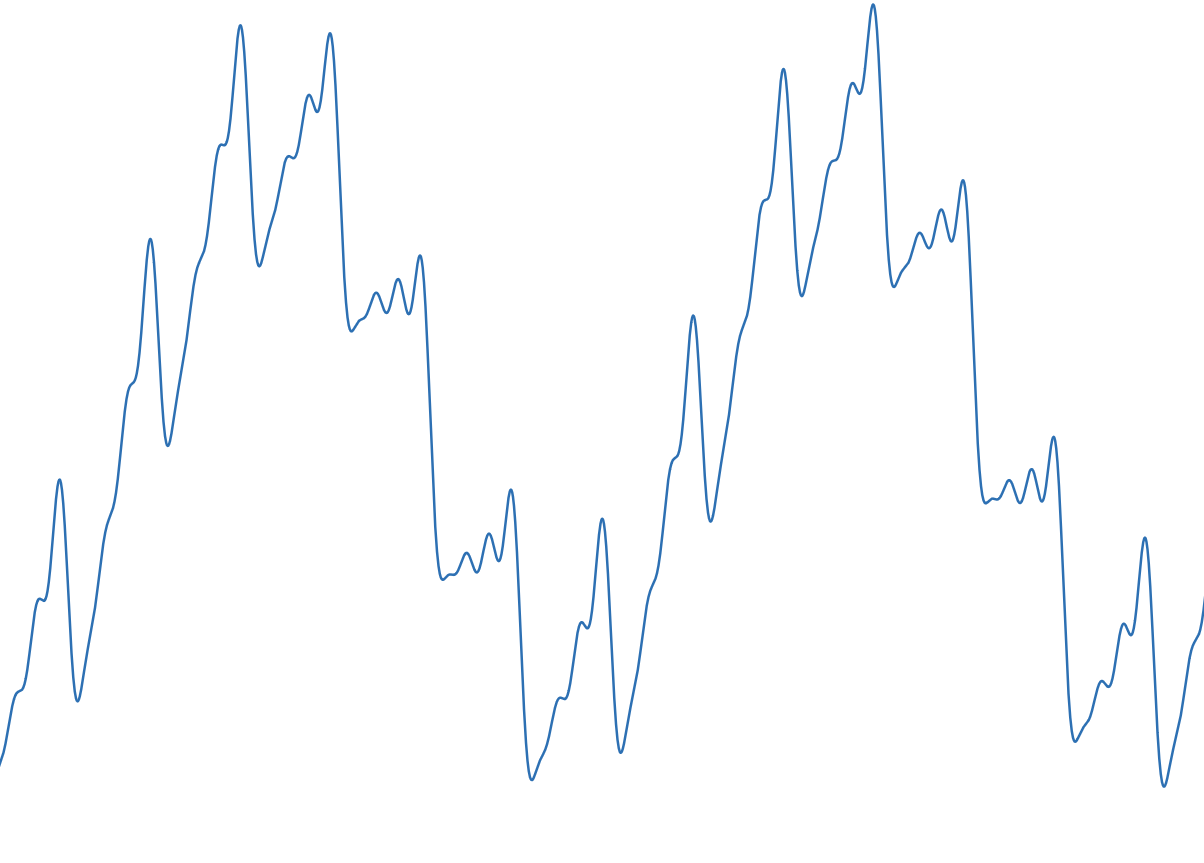
\includegraphics[width=0.7\textwidth]{soundwave.png}
    \caption{A sound wave.}
    \label{fig:soundwave}
\end{figure}

Since figure \ref{fig:soundwave} a pure mathematical function, it has infinite precision. At any given point of infinitely precision, the function is guaranteed to have a value. This is called \textbf{analog} data, because it is not given in discrete points, it is given as a smooth curve.

In order to convert this into digital data (represented in binary), it must pass through an Analog to Digital converter. This approximates the function into discrete data points. This device takes points on the curve at regular intervals and stores their height. Therefore, after the sound wave mentioned above passes through an ADC, it may look as follows:

\vfill

\begin{figure}[H]
    \centering
    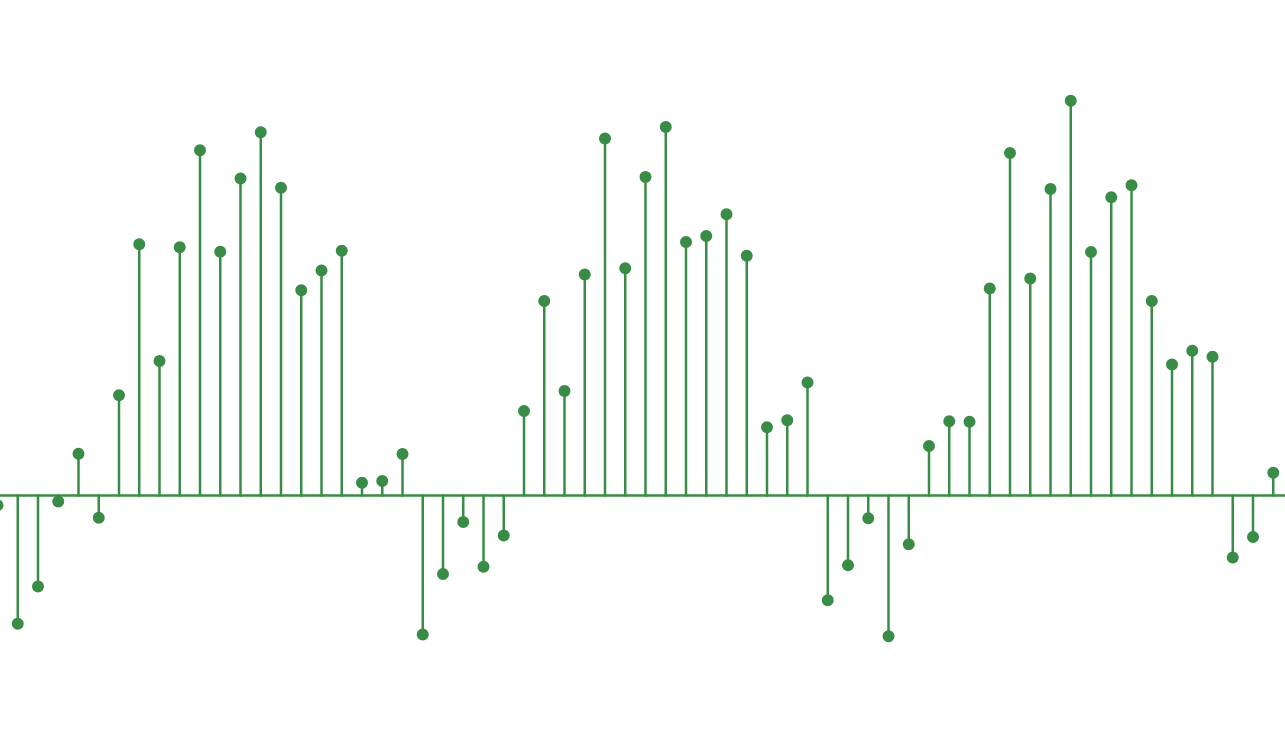
\includegraphics[width=0.7\textwidth]{soundwave_sampled.png}
    \caption{The sound wave, but sampled (now discrete)}
    \label{fig:soundwave_sampled}
\end{figure}

with points being placed on the curve. Each one of those points' data values can now be stored in binary, like {\mono 1001}\footnote{in math terms, this is now a discrete function, as there are only some values at which the function is defined}. 

The \textbf{sampling resolution} is how accurate each one of the points are. If the sampling resolution is low (4 bytes), the range of data it can be in binary is low, meaning less accuracy. However, if the sampling resolution is high (44,100 bytes), each data point stored is much more accurate.

The \textbf{sampling rate} is how often these data points are taken. The diagram below illustrates this.

\vfill

\textit{(turn over)}

\begin{figure}[H]
    \centering
    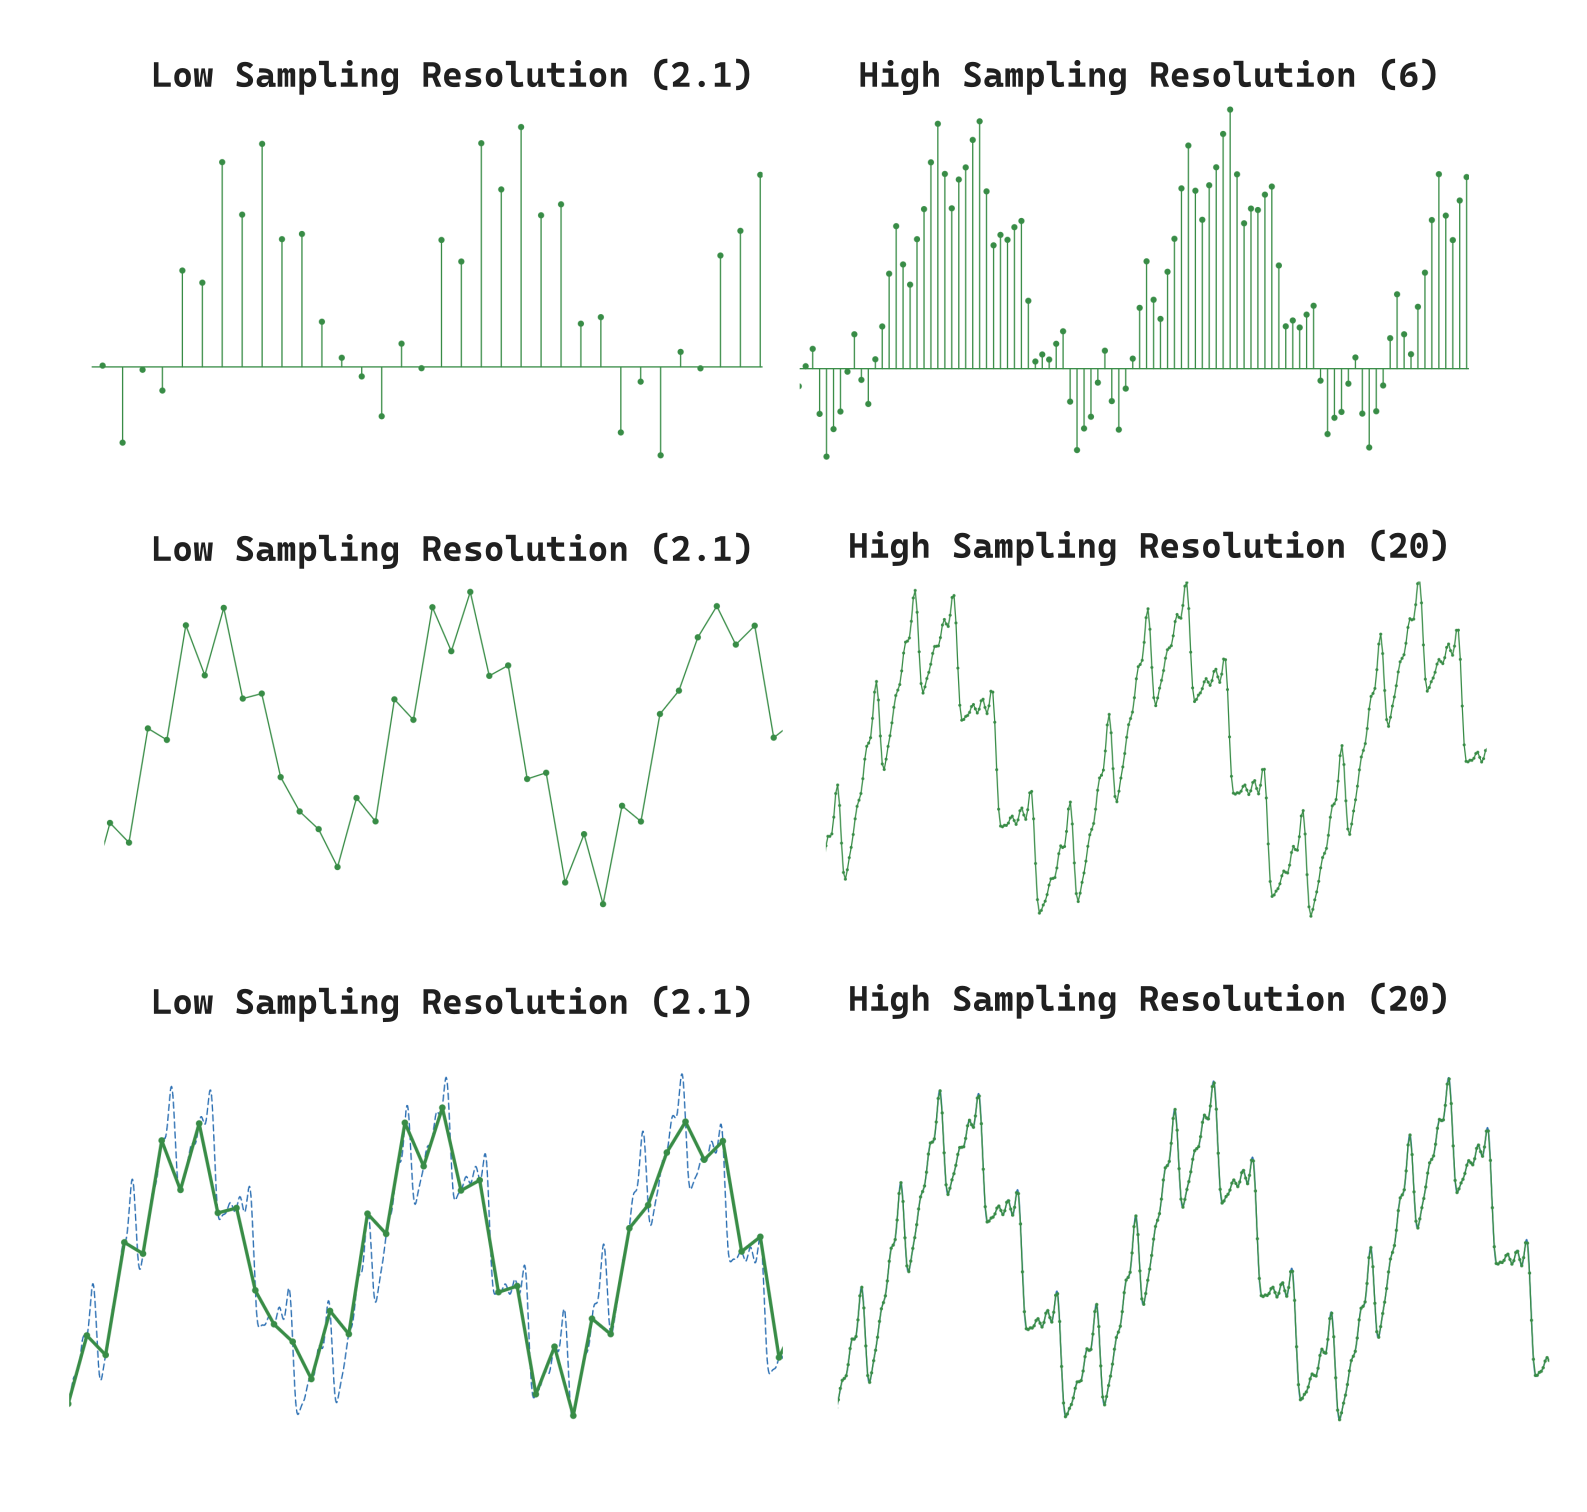
\includegraphics[width=\textwidth]{sampling.png}
    \caption{Sampling resolution}
    \label{fig:sampling}
\end{figure}

The first row of figure \ref{fig:sampling} demonstrates the difference between a badly sampled wave and a well sampled wave. The second row are the same points, but they are connected together; showing that the sampling rate affects the accuracy. The third row proves this. The blue line is the original function; the low sampling rate example does not approximate the function well, but on the high sampling rate example, one cannot see the blue line, as it is approximated so well.

\begin{figure}[H]
    \centering
    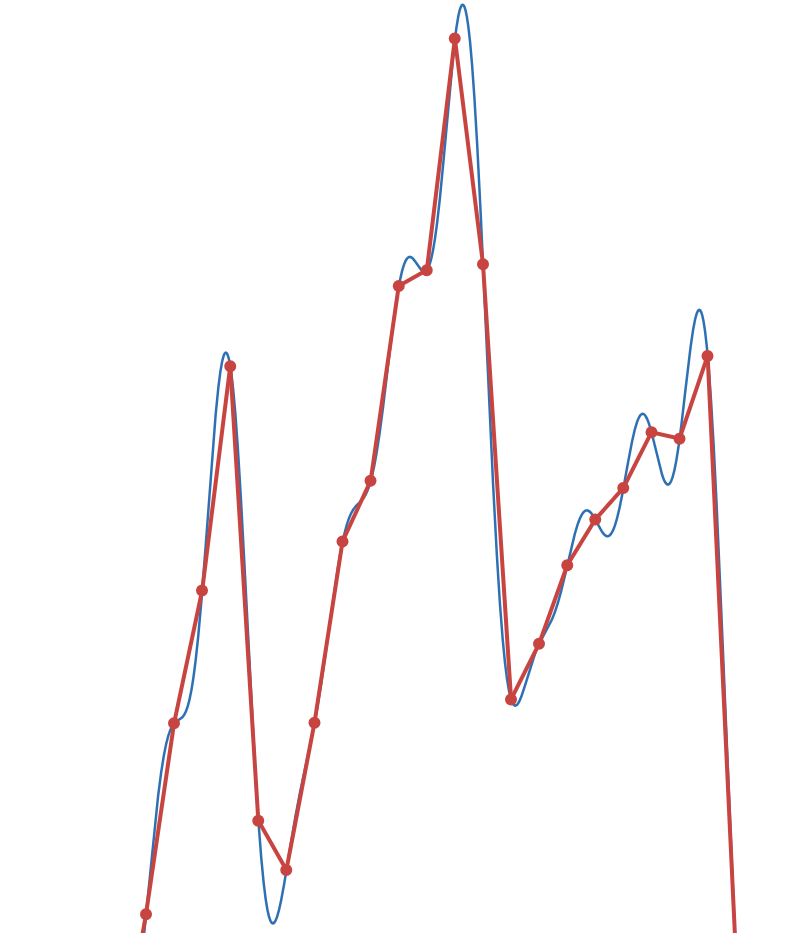
\includegraphics[width=0.5\textwidth]{sampling_zoomed.png}
    \caption{A zoomed in rendition of the sound wave.}
    \label{fig:sampling_zoomed}
\end{figure}

Sampling is never perfect, and can never mimic the nature of a continuous function. Figure \ref{fig:sampling_zoomed} shows the curve with a sample rate of 8.5.

Finally, the \textbf{sample size} is how long the sample is; the length of the wave captured.

\textbf{What all this means for a computer and human} is that an audio file with a low sampling rate and resolution will sound worse (granier, less clear) as the curve is not approximated as well. An audio file with a higher sampling rate and resolution will sound better (clearer).

To calculate the file size, perform (everything except explicitly mentioned is in bytes):

{\centering\mono
file size = sample size * sampling resolution * sampling rate (Hz)
}

\textit{NOTE: All the images were generated with \href{https://www.desmos.com/calculator/qlduxmdckb}{this} desmos chart\footnote{link: \url{https://www.desmos.com/calculator/qlduxmdckb}}. Please play around with it! It teaches you a lot.}

\newpage
\subsection{Images}

Images are actually represented as a grid of pixels. Each pixel can hold a color value. Consider this black and white image:

\begin{figure}[H]
    \centering
    
\includegraphics[width=0.3\textwidth]{8x8image.png}
    \caption{An 8x8 black-and-white grid}
    \label{fig:8x8image}
\end{figure}

Figure \ref{fig:8x8image} is a black-and white image. Let us suppose that each black pixel is represented as a 1 and each white is represented as a 0. In binary, the image would be represented as follows:

\medskip

{\mono\centering
    0 0 0 0 0 0 0 0\\
    0 1 1 1 1 1 1 0\\
    0 1 0 0 0 0 1 0\\
    0 1 0 1 1 0 1 0\\
    0 1 0 1 1 0 1 0\\
    0 1 0 0 0 0 1 0\\
    0 1 1 1 1 1 1 0\\
    0 0 0 0 0 0 0 0\\
}

\medskip
\begin{figure}[H]
    \centering
    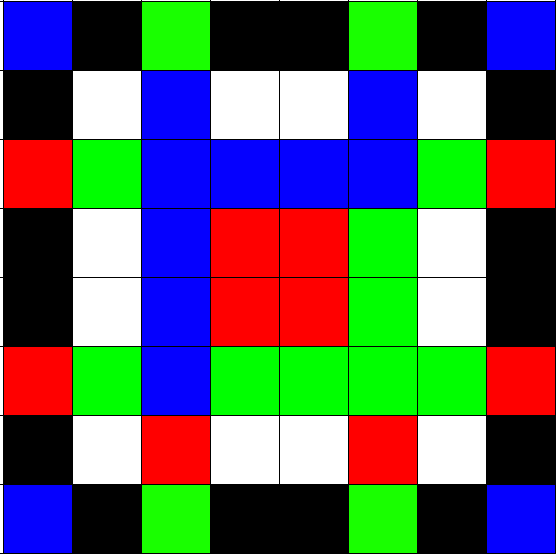
\includegraphics[width=0.3\textwidth]{8x8colorimage.png}
    \caption{An 8x8 color "image"}
    \label{fig:8x8colorimage}
\end{figure}

Now let us represent \ref{fig:8x8colorimage} in binary. We will now assume that black is 0 (the absence of color), 1 is red, 2 is green, 3 is blue and 4 is white. The representation now becomes:

\newpage 

{\mono\centering
    3 0 2 0 0 2 0 3\\
    0 4 3 4 4 3 4 0\\
    1 2 3 3 3 3 2 1\\
    0 4 3 1 1 2 4 0\\
    0 4 3 1 1 2 4 0\\
    1 2 3 2 2 2 2 1\\
    0 4 1 4 4 1 4 0\\
    3 0 2 0 0 2 0 3\\
}

\medskip

The number of bytes used to store one pixel of data is called the \emph{bit depth}. Since we used 0, 1, 2, 3, 4 to represent our image, we actually need a whole 8 bits or 1 byte to represent each pixel. This means that the bit depth is one byte (which gives us 8 colors). The resolution of figure \ref{fig:8x8colorimage} is the size of the image, which is 8x8 pixels, meaning 64 in total. As the resolution increases, more data can be held. To calculate the file size, perform:

{\centering\mono
file size (bytes/bits) = pixels wide * pixels high * bit depth (bytes/bits)
}

For us, it gives us 64 bytes of used space.

A higher resolutions means that images look sharper. Provided is an image from the textbook showing 5 images of the same wheel with varying resolutions. 

\begin{figure}[H]
    \centering
    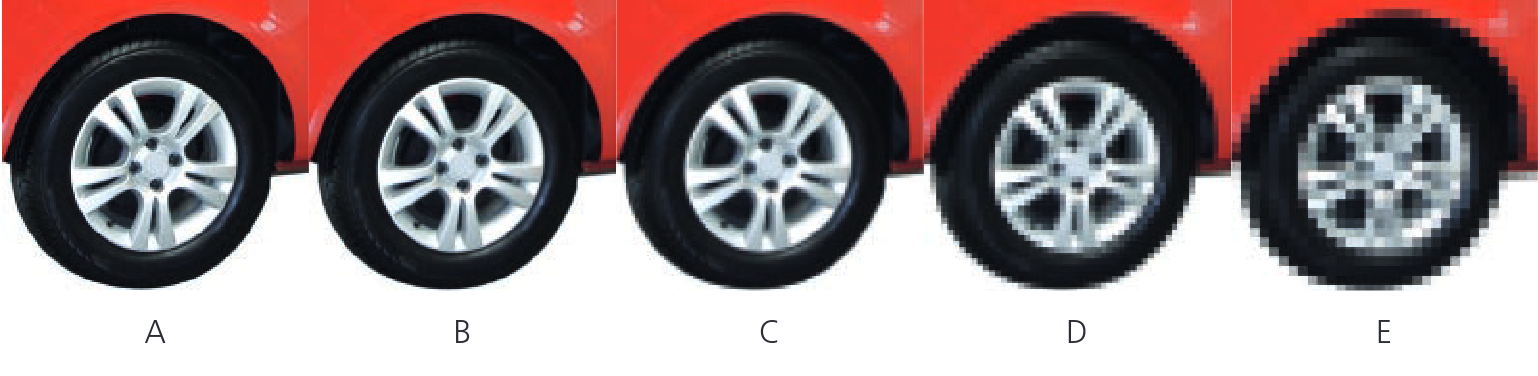
\includegraphics[width=0.8\textwidth]{wheels.png}
    \caption{From the textbook: Five images of the same car wheel using different resolutions.}
    \label{fig:wheel}
\end{figure}

Image A is the sharpest-looking in figure \ref{fig:wheel}, as it has more pixels than, say, Image E to store the same data. Therefore, it looks better.

\end{document}
